\Chapter{Tervezés}

Van egy eredeti problémánk, melyben tényezőink a tantárgyak, tantermek, tanárok és 
osztályok. Mindenképpen szükség van ennek a felbontására, hogy egyszerűbb részproblámákat kapjunk, melyek megoldhatóak hagyományos algoritmusokkal, illetve hagyományos optimalizálási módszerekkel és együttesen alkotják az órarendgenerálási probléma megoldását. A genetikus algoritmust a plusz feltételeknek lehető legjobban megfelelő órarendek megkapásához fogjuk használni, merthogy ez hagyományos módszerekkel nem megoldható. Ezt onnan lehet tudni, hogy nem tudjuk matematikailag leírni a szükséges algoritmust. A plusz feltételek azok a feltételek, melyek nélkül is érvényes és elfogadható, de nem feltétlenül kielégítő órarendeket kapunk. Ezek lesznek a kora reggeli/késő délutáni órák számának minimalizálása, a napi óraszámok arányos eloszlása/pénteki órák számának minimalizálása, illetve a részmunkaidős tanárok beosztása.

\Section{Teremhozzárendelési feladat}

Az első részfeladat a teremhozzárendelési, amely kétfázisú lesz. Az első fázisban osztályokat kell hozzárendelni optimálisan a tantermekhez. Ez egy halmazfelbontási feladat, ahogyan az optimalizálásban nevezzük, ami arról szól, hogy az egyik halmaz (osztályok) és másik halmaz (tantermek) elemeihez 1:1 hozzárendelést kell elvégezni, vagyis minden osztályhoz pontosan 1 tanteremnek kell tartoznia és minden tanteremhez pontosan 1 osztálynak. Mindezt úgy, hogy a legoptimálisabb megoldást kapjuk a kihasználatlanság minimalizálásának szempontjából, mert így elkerülhetjük azt, hogy egy osztály terem nélkül maradjon, miközben létezik olyan hozzárendelés, hogy minden osztálynak jusson terem \cite{nagy1998operaciokutatas}. A kihasználatlanság az adott terem kapacitásának és az adott osztály létszámának a különbsége. Természetesen amennyiben van olyan osztály, amelynek létszáma nagyobb, mint bármely terem befogadóképessége, vagy több olyan, adott létszámot elérő osztály van, mint ahány terem, amelyik rendelkezik az adott befogadóképességgel, akkor a feladat nem megoldható, így legelőször ezzel kapcsolatban kell ellenőrzést végezni. Feltétel nyilván, hogy egy osztálynak nem lehet órája olyan teremben, amelynek a kapacitása kisebb az osztály létszámánál, ezenkívül egy évfolyam osztályai és az évfolyamon képzett nyelvi, fakultációs vagy egyéb csoportok esetében megengedett ugyanannak a teremnek a hozzárendelése. A második
fázis azért szükséges, mert egyes termek lehetnek elsősorban adott tantárgy(ak) számára fenntartottak). Itt már nem osztályokat, hanem osztály-tantárgy kettősöket veszünk ("táblázatos" forma), vagyis minden osztályt annyiszor kell számba venni, ahány tantárgy tartozik hozzá. 

\SubSection{Formalizálás}

\begin{itemize}
	\item $n \in \Bbb{N}$: osztályok száma
	\item $m \in \Bbb{N}$: tantermek száma
	\item $p \in \Bbb{N}$: osztály-tantárgy kettősök száma
	\item $l \in \Bbb{N}^n$: osztályok létszáma
	\item $k \in \Bbb{N}^m$: tantermek kapacitása
	\item $h \in \Bbb{N}^n$: termek száma, ahová az egyes osztályok beférnek
	\item $C \in \Bbb{N}^{n \times m}$: költségmátrix
	\item $A \in \{0;1\}^{n \times m}$: párosításmátrix
	\item $X \in \{0;1\}^{n \times m}$: hozzárendelés-mátrix
\end{itemize}

\[
C_{ij} =
\begin{cases}
k_j-l_i, & \hbox{ha } X_{ij}=1, \\
\infty & \hbox{egyébként}.
\end{cases}
\]

\[
A_{ij} =
\begin{cases}
1, & \hbox{ha } l_i \leq k_j, \\
0& \hbox{egyébként}.
\end{cases}
\]

\[
X_{ij} =
\begin{cases}
1, & \hbox{ha az $i$-edik osztálynak a $j$-edik teremben lesz a tanóra}, \\
0&
\hbox{egyébként}.
\end{cases}
\]

$$\sum_{j=1}^m C_jX_j \rightarrow \hbox{min}$$

$$\sum_{j=1}^m A_{ij}X_j=1$$

$$i=1, 2, \ldots, n$$

$$j=1, 2, \ldots, m$$

\SubSection{Időbonyolultság}

Összes lehetséges esetek száma:

$$P=\prod_{i=1}^n h_i$$
Összes lehetséges megoldások száma:

$$P=\prod_{i=1}^n h_i-(i-1)$$
Nézzük az összes lehetséges esetek és lehetséges megoldások számát az alapesetben, az eredeti példa esetén,
illetve évfolyamonként 6, 7, 8 osztályra kibővített esetben (ahol a termek számát plusz egy évfolyamonkénti osztály
esetén 5-tel növeltem) (\ref{tab:complexity3}. táblázat).

\begin{table}[h!]
	\centering
	\caption{Az esetek és megoldások száma a tanárok számának függvényében}
	\label{tab:complexity3}
	\medskip
\begin{tabular}{|l|c|c|c|c|}
\hline
& 5 & 6 & 7 & 8 \\
\hline
Összes esetek & $1,1 \cdot 10^{23}$ & $1,4 \cdot 10^{31}$ & $1,7 \cdot 10^{38}$ & $2 \cdot 10^{46}$ \\ 
\hline
Összes megoldások & $5,3 \cdot 10^{16}$ & $3,5 \cdot 10^{22}$ & $1,5 \cdot 10^{26}$ & $3,3 \cdot 10^{31}$ \\
\hline
\end{tabular}
\end{table}

A teremhozzárendelések vizsgálata kapcsán a becsült bonyolultságokat \aref{fig:teremhozzarendeles}. ábrán láthatjuk.

\begin{figure}[h!]
	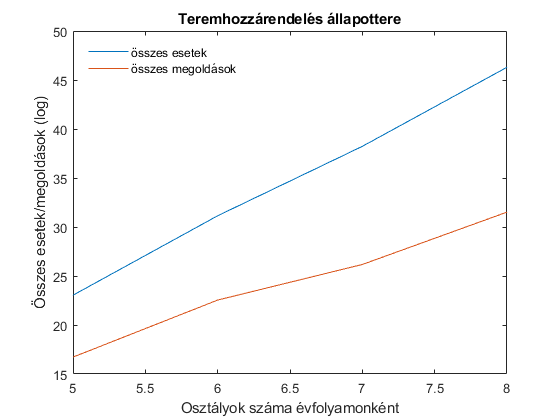
\includegraphics[width=\linewidth]{images/teremhozzarendeles.png}
	\caption{Teremhozzárendelés állapottere}
	\label{fig:teremhozzarendeles}
\end{figure}

Az első fázis növekedési rendje a következő: $T(n,m)=\ \sim \ \Theta (2nm).$

A második fázis növekedési rendje: $T(n,m,p)=\ \sim \ \Theta (np+mp).$

Növekedési rend: $T(n,m,p)=\ \sim \ \Theta (2nm+np+mp).$

A saját példám futási idejének tudatában, a növekedési rendet felhasználva ki tudtam számolni, hogy milyen futási időre számíthatnánk a Miskolci Egyetem esetében. Az én példámban 30 terem, 30 tanár, 60 osztály, 220 osztály-tantárgy kettős és 40 időablak van, míg a Miskolci Egyetem esetében becsült adatokként 200 terem, 500 tanár, 1000 osztály, 2000 osztály-tantárgy kettős és 30 időablak. Azt kaptam, hogy $2min$ $23sec$ az átlagosan várható futási idő, a Miskolci Egyetem esetében, IntelCore i7 875K processzorral. Amely processzor 92100 műveletet végez másodpercenként.

\Section{Tanárhozzárendelési feladat}

Az osztály-tantárgy kettősökhöz immáron a tanárokat rendeljük hozzá. Ez egy halmazlefedési feladat, ami abban különbözik a halmazfelbontásitól, hogy 1:N hozzárendelés van, ugyanis egy tanárhoz több osztály-tantárgy kettőst is rendelhetünk, sőt ugye kell is többet hozzárendelni. A párosításmátrixban két feltételtől is függ, hogy 0 vagy 1 kerül a rublikába. Egyrészt, hogy az adott tanár tudja-e tanítani az adott tantárgyat, másrészt hogy az adott osztálynak van-e ilyen tárgya \cite{nagy1998operaciokutatas}. A minimalizálás pedig itt arra vonatkozik, hogy minél kisebb legyen a tanárok heti óraszámai közötti eltérés, ne fordulhasson elő, hogy mondjuk míg valaki 30 órát tart egy héten, addig más 5-öt.
A futtatás után kapott eredményt látva megállapítható, hogy amennyire lehetett, sikerült kiküszöbölni a tanárok egyenlőtlen terhelését, megkaptuk a lehető legoptimálisabb, olyan hozzárendelés-mátrixot, amely meghatározza, hogy egy adott osztálynak egy adott tantárgyat, melyik tanár tartsa.

\SubSection{Formalizálás}

\begin{itemize}
	\item $n$: osztály-tantárgy kettősök száma
	\item $m$: tanárok száma
	\item $p$: tantárgyak száma
	\item $u \in \Bbb{N}^p$: az egyes tárgyakat hallgató osztályok száma
	\item $v \in \Bbb{N}^p$: az egyes tárgyakat oktató tanárok száma
	\item $t \in \Bbb{N}^m$: tanárok heti óraszáma
	\item $o \in \Bbb{N}^n$: osztály-tantárgy kettősök heti óraszáma
	\item $A \in \{0;1\}^{n \times m}$: párosításmátrix, $A_{ij} = 1$, ha az $i$-edik osztály-tantárgy kettősben szereplő tantárgyat tudja tanítani a $j$-edik tanár, egyébként 0.
	\item $X \in \{0;1\}^{n \times m}$: hozzárendelés-mátrix, $X_{ij} = 1$, ha az $i$-edik osztály-tantárgy kettősben szereplő osztálynak az ugyanezen kettősben szereplő tantárgyat a $j$-edik tanár fogja tartani, egyébként 0.
\end{itemize}

\[
t_{j} =
\begin{cases}
t_j+o_i,& \hbox{ha } X_{ij}=1, \\
t_j & \hbox{egyébként}.
\end{cases}
\]

$$\sum_{j=1}^m \vert o_jX_j-\overline{o}\vert \rightarrow \hbox{min}$$

$$\sum_{j=1}^m A_{ij} X_j=1$$

$$k=1, 2, \ldots, p$$

\SubSection{Időbonyolultság}

Összes esetek száma:

$$P=m^n.$$
Összes megoldások száma:

$$P=\prod_{k=1}^p v_k^{u_k}.$$

Az esetek és megoldásoknak a számát az osztályok számának függvényében \aref{fig:tanarhozzarendeles}. ábrán lévő grafikonon láthatjuk szemléltetve.

\begin{figure}[h!]
	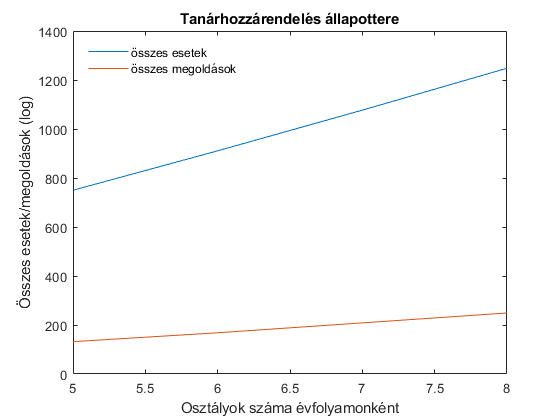
\includegraphics[width=\linewidth]{images/tanarhozzarendeles.png}
	\caption{Tanárhozzárendelés állapottere}
	\label{fig:tanarhozzarendeles}
\end{figure}

A lehetséges esetek és megoldások száma közötti összefüggésre néhány becslést láthatunk \aref{tab:complexity}. táblázatban. (A tanárok számát plusz egy évfolyamonkénti osztály esetén 3-mal növeltem.)

\begin{table}[h!]
	\centering
	\caption{Az esetek és megoldások száma a tanárok számának függvényében}
	\label{tab:complexity}
	\medskip
\begin{tabular}{|l|c|c|c|c|}
\hline
& 5 & 6 & 7 & 8 \\
\hline
Összes esetek & $9,3 \cdot 10^{325}$ & $6,5 \cdot 10^{395}$ & $7,8 \cdot 10^{467}$ & $9,2 \cdot 10^{541}$ \\
\hline 
Összes megoldások & $1,1 \cdot 10^{132}$ & $2 \cdot 10^{168}$ & $4,2 \cdot 10^{208}$ & $1,2 \cdot 10^{249}$ \\
\hline
\end{tabular}
\end{table}

Növekedési rend: $T(n,m)=\Theta (nm+nm^2).$

A növekedési rend értelmében $4min$ $29sec$ az átlagosan várható futási idő, a Miskolci Egyetem esetében, IntelCore i7 875K processzorral. 

\Section{Időablakok beosztása}

Ennek lényege, hogy a korábbiak alapján kapott osztály-tantárgy-terem-tanár
hozzárendeléseket ütközésmentesen beosszuk időablakokba. Merthogy egy időablakban nyilván nem szerepelhet többször ugyanaz az osztály, ugyanaz a terem és ugyanaz a tanár sem. Egy időablak legfeljebb annyi hozzárendelést tartalmazhat, amennyi a tanárok száma. Amire még oda kell figyelni, hogy egy osztály-tantárgy kettős annyiszor forduljon elő, amennyi a heti óraszáma az adott osztálynak az adott tárgyból.

\SubSection{Formalizálás}

\begin{itemize}
	\item $n \in \Bbb{N}$: osztály-tantárgy kettősök száma
	\item $m \in \Bbb{N}$: tanárok száma
	\item $p \in \Bbb{N}$: tantermek száma
	\item $r \in \Bbb{N}$: időablakok száma
	\item $o \in \Bbb{N}^n$: osztály-tantárgy kettősök heti óraszámai
	\item $c \in \Bbb{N}^n$: osztály-tantárgy kettősök előfordulásainak száma
	\item $e \in \Bbb{N}^m$: tanárok előfordulásainak száma
	\item $h \in \Bbb{N}^p$: tantermek előfordulásainak száma
\end{itemize}

$$\sum_{i=1}^n c_i \in (0,1), \quad \hbox{minden }l\hbox{ időablak esetén.}$$

$$\sum_{j=1}^m e_j \in (0,1), \quad \hbox{minden }l\hbox{ időablak esetén.}$$

$$\sum_{k=1}^p h_k \in (0,1), \quad \hbox{minden }l\hbox{ időablak esetén.}$$

$$\sum_{i=1}^n \vert o_i - c_i \vert = 0$$

$$l=1, 2, \ldots, r$$

\SubSection{Időbonyolultság}

Összes esetek száma:

$$P=\binom{n+m-1}{m}.$$

Összes megoldások száma:

$$P=\binom{n}{m}.$$
A lehetséges esetek és megoldások száma (\ref{tab:complexity2}. táblázat). (A tanárok számát plusz egy évfolyamonkénti osztály esetén 3-mal növeltem.)

\begin{table}[h!]
\centering
\caption{A lehetséges esetek és megoldások száma}
\label{tab:complexity2}
\medskip
\begin{tabular}{|l|c|c|c|c|}
\hline
& 5 & 6 & 7 & 8 \\
\hline
Összes esetek & $5 \cdot 10^{105}$ & $9,1 \cdot 10^{119}$ & $1,7 \cdot 10^{134}$ & $3,5 \cdot 10^{148}$ \\
\hline 
Összes megoldások & $8,9 \cdot 10^{36}$ & $6,8 \cdot 10^{41}$ & $4,5 \cdot 10^{46}$ & $2,7 \cdot 10^{51}$ \\
\hline
\end{tabular}
\end{table}

A kapott eredményeket \aref{fig:idoablak}. ábrán láthatjuk szemléltetve.

\begin{figure}[h!]
	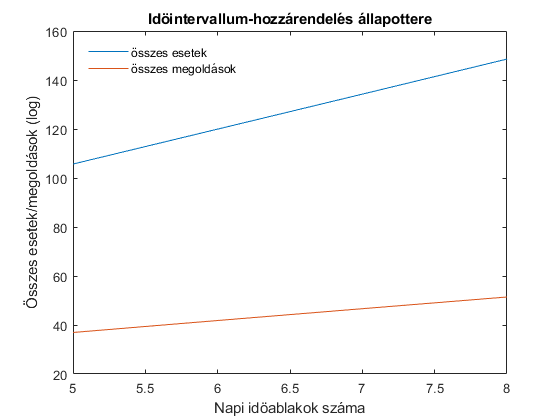
\includegraphics[width=\linewidth]{images/idoablak.png}
	\caption{Időablakbeosztás állapottere}
	\label{fig:idoablak}
\end{figure}

Növekedési rend: $T(n,m,r)=\ \sim \ \Theta(nmr)$.

A növekedési rend értelmében $6min$ $15sec$ az átlagosan várható futási idő, a Miskolci Egyetem esetében, IntelCore i7 875K processzorral. 

\Section{Időintervallumok hozzárendelése}

A megkapott időablakok még nincsenek időintervallumhoz kötve, bármelyik felcserélhető bármelyikkel. Azt a feladatot, hogy a megadott plusz feltételek alapján optimális megoldást találjunk, vagyis mely időablak mely időintervallumba kerüljön, a genetikus algoritmus végzi el nekünk.

\SubSection{Probléma modellezése}

\noindent A probléma leképezése a genetikus algoritmus összetevőire:

\begin{itemize}
	\item \textbf{gén:} Egy konkrét, általános- és középiskolák esetén egy óra hosszúságú, 	          főiskolák/egyetemek esetén két óra hosszúságú időintervallum. Implementációja szótár, két elemmel: nap (enum) és a napon belüli időablak (string).
	\item \textbf{egyed:} Az összes időablak sorrendje, az egyedek mibenlétét a gének sorrendje határozza meg. Implementációja szintén szótár, elemei a gének listája, a cél\-függ\-vény-érték és az
	egyedi azonosító.
	\item \textbf{populáció:} Az egyedek összességét tárolja, melyeknek számát a programozó állapítja meg, a hatékonysági tesztek által. Implementációja lista.
	\item \textbf{célfüggvény:} Esetemben a kora reggeli/késői délutáni órák számát akarom minimalizálni, illetve a napi óraszámok arányos eloszlása/pénteki órák számának minimalizálása is szempont. Minden tanárhoz tartozik egy \textsl{balance} és egy \textsl{extremisms} érték,
	melyet a felhasználó ad meg és ezzel skálán rögzíti mennyire fontosak/kevésbé fontosak ezek a különböző szempontok az adott tanároknak. Ezek az értékek adják a célfüggvény súlyozását, melynek értéke ennek megfelelően minden problémás időintervallum esetén növekszik. Minél kisebb a célfüggvény értéke, az egyed annál megfelelőbb.
	\item \textbf{szelekció:} Rátermettség-arányos választással, súlyozott random generátornak köszönhetően. Miután a populáció egyedeit a célfüggvény-értékek alapján sorrendbe rakta a rendező metódusunk, a súlyozott random generátor annak megfelelő valószínűséggel szelektálja ki szülőnek az egyedeket, amilyen helyezést foglalnak el a listán. Ahány egyedből áll a populáció, a legmegfelelőbb egyednek annyiszor nagyobb esélye lesz, mint a leggyengébb egyednek. Amire még oda kell figyelni, hogy ugyanaz az egyed ne kerülhessen kétszer is kiválasztásra a szülők meghatározásakor, mivel az azt jelentené hogy a gyerek anyja egyben az apja is (igaz, a South Park rajzfilmsorozatban találkozhatunk ilyennel)...
	\item \textbf{keresztezés:} Egypontos keresztezéssel. Véletlenszám-generálással döntjük el, hol legyen a keresztezési pont. A nehézséget annak megoldása jelenti, hogy ugyanaz az időablak (vagyis ugyanaz a gén) ne fordulhasson elő többször a gyermek egyedben.
\end{itemize}

\SubSection{Formalizálás}

\begin{itemize}
	\item P: populáció mérete
	\item G: generációk száma
	\item I: időablakok száma
	\item $n \in \Bbb{N}$: osztály-tantárgy kettősök száma
	\item $m \in \Bbb{N}$: tanárok száma
	\item $o \in \Bbb{N}$: osztály-tantárgy kettősök heti óraszámai
	\item $b \in \{1;5\}$: tanárok \textit{balance} értékei
	\item $e \in \{1;5\}$: tanárok \textit{extremisms} értékei
	\item $c: \Bbb{N} \rightarrow \Bbb{N}$: célfüggvény
\end{itemize}

$$ c=\sum_{j=1}^m \sum_{l=1}^I \quad
\begin{cases}
b_j, & \hbox{ha a \textit{balance} feltétel teljesül }l\hbox{ időablakban,}\\
e_j, & \hbox{ha a \textit{extremisms} feltétel teljesül }l\hbox{ időablakban,}\\
b_j+e_j, & \hbox{ha az előző két feltétel egyszerre teljesül},\\
0 & \hbox{egyébként.}
\end{cases}
$$

$$
c \rightarrow min
$$

\SubSection{Időbonyolultság}

Összes esetek száma:

$$P=I^I.$$
Összes megoldások száma:

$$P=I!$$
A számszerűsített példában itt nem évfolyamonkénti osztályok száma lesz, hanem napi időablakok száma. Az egyetemek/főiskolák kapcsán 6 (egy dupla óra egy időablak), az általános iskolák kapcsán 7, a középiskolák kapcsán pedig 8 időablakkal számolunk. Hangsúlyozom, hogy ez csak példa, a felhasználó mást is megadhat (\ref{tab:complexity3}. táblázat).

\begin{table}[h!]
	\centering
	\caption{A lehetséges esetek és megoldások száma}
	\label{tab:complexity3}
	\medskip
\begin{tabular}{|l|c|c|c|}
\hline
& 6 & 7 & 8 \\
\hline
Összes esetek & $46656$ & $823543$ & $16777216$ \\
\hline 
Összes megoldások & $720$ & $5040$ & $40320$ \\
\hline
\end{tabular}
\end{table}

A kapott, bonyolultság vizsgálatával kapcsolatos eredményeket \aref{fig:idointervallum}. ábrán láthatjuk.

\begin{figure}[h!]
	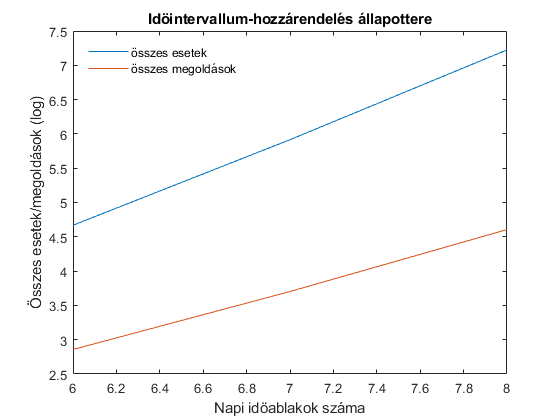
\includegraphics[width=\linewidth]{images/idointervallum.png}
	\caption{Időintervallum-hozzárendelés állapottere}
	\label{fig:idointervallum}
\end{figure}

Célfüggvény növekedési rendje: $T(n,m,o)=\Theta(nmo)$.

Keresztezés növekedési rendje: $T(I)=\ \sim \ \Theta(I^2)$.

Hozzájön még ehhez a tiszta öröklődés, a mutáció és a rendező metódus növekedési rendje, de ezek elhanyagolhatóak. A tiszta öröklődés és a mutáció egyetlen rövid ciklusból áll, ami egy csupán 30-40 elemű listán iterál végig, a minimum rendezés növekedési rendje pedig ugyan négyzetes, de csak generációnként egyszer kerül meghívásra.

Növekedési rend: $T(P,G,I,n,m,o)=\ \sim \ \Theta(G \cdot P \cdot (nmo+I^2))$.

A tesztelés során az derült ki, hogy átlagosan 48 generációra van szükség, így a növekedési rend értelmében 48 perc 25 másodperc az átlagosan várható futási idő, a Miskolci Egyetem esetében, IntelCore i7 875K processzorral. Ha vannak részmunkaidős tanárok és ezért vizsgáljuk, illetve büntetjük az ezzel kapcsolatos értékeket is a célfüggvényben, akkor néhány másodperccel több.

Könnyen belátható, hogy a célfüggvény és azon belül a tanárokon végigiteráló ciklus "dobja meg" a futási időt. Amennyiben nem adunk rá lehetőséget minden tanárnak, hogy a saját \textit{balance} és \textit{extremisms} értékeivel rendelkezzen, hanem egységesen állítjuk be ezeket az értékeket/alapértelmezett értékkel számolunk, akkor kevesebb mint 5 másodperc lesz a futási idő. Amennyiben adunk, az sem jelent nagy problémát, főleg ha szervergéphez méltó, az enyémtől 2$\times$, 3$\times$ nagyobb teljesítményű processzorral rendelkezünk.

Maga a generálás (a szűkebb értelemben vett generálás) a \textit{generator.py} modul algoritmusai által történik, 11 másodperc futási ideje azonban jelentéktelen. Az én processzorommal az egész órarendgenerálási folyamat átlagosan várható futási ideje, összesen 61 perc 43 másodperc tanáronkénti \textit{balance} és \textit{extremisms} értékek esetén, egységes értékek esetén pedig 13 perc 23 másodperc. Ha a tanárokat manuálisan akarja hozzárendelni az osztályokhoz a felhasználó, akkor még kevesebb, mivel ebben az esetben a tanárhozzárendelési feladatot nem kell végrehajtani. Kijelenthetjük, hogy nem létezik olyan méretű oktatási intézmény, melynek esetében ne tudnának belátható időn belül eredményt szolgáltatni az algoritmusaim.

